
\begin{frame}{Why watermark a language model?}
    \begin{figure}
        \centering
        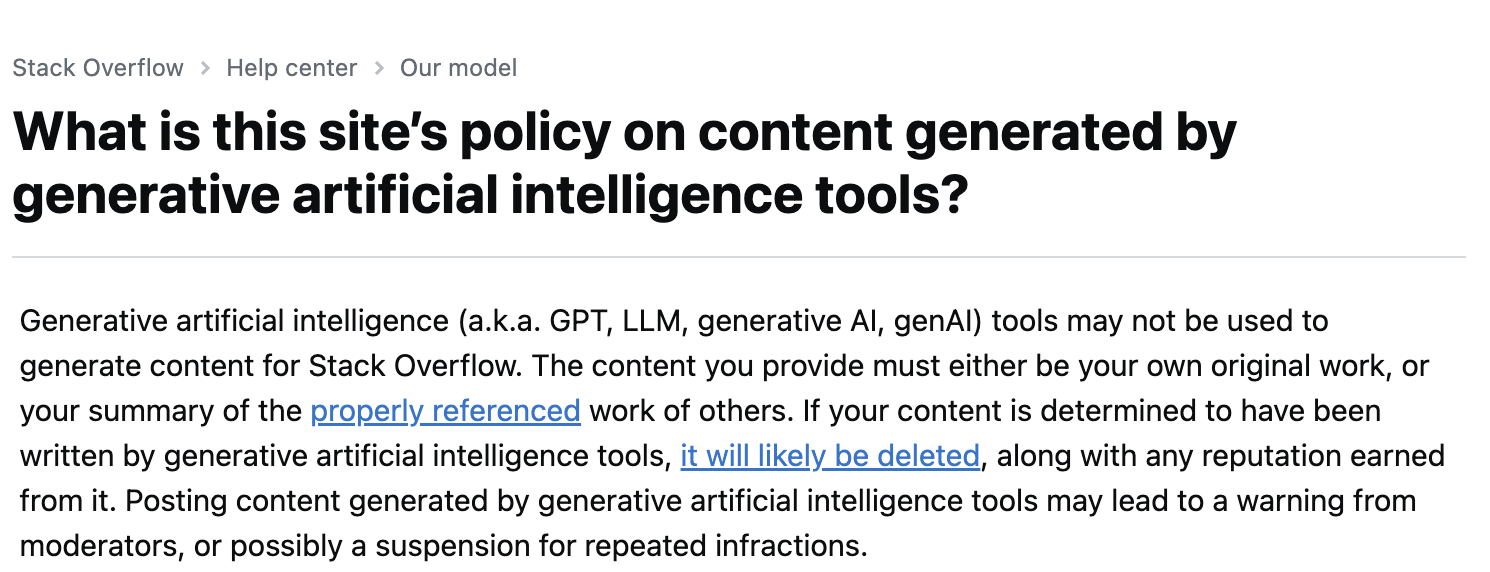
\includegraphics[width=0.8\linewidth]{./images/so-gen-ai-policy.png}
        \caption{\footnotesize Screenshot of the Stack Overflow generative AI policy\cite{so-gen-ai-policy}.}
        \label{fig:so-policy}
    \end{figure}
\end{frame}

\begin{frame}{Why watermark a language model?}
    \begin{itemize}
        \item Large language models can mass-produce human-like text, raising concerns about \emph{provenance}\footnote{a record of ownership of a work of art or an antique, used as a guide to authenticity or quality}.
        \item The increased usage of LMs can lead to issues in academic integrity, plagiarism, copyright infringement and the propagation of misinformation
        \item Platforms and developers of LMs want to track (mis)use of their models.
        \item Can improve future LM training, as text generated by LMs can be removed from the training set.
    \end{itemize}
\end{frame}

\begin{frame}{What is watermarking?}
    \begin{itemize}
        \item A \textbf{watermark} is a hidden signal embedded in generated text that encodes its source. This signal can be detected later to prove the text's origin.
        \item The watermarking protocol described by \emph{Kuditipudi et al.} involves three parties:
              \begin{enumerate}
                  \item \textbf{LM Provider:} Generates text with a secret watermark (using a secret key).
                  \item \textbf{User:} Receives the watermarked text. They might publish it or attempt to \textit{edit it to evade detection}.
                  \item \textbf{Detector:} Uses the shared secret key to verify if given text carries the watermark (hence came from the provider).
              \end{enumerate}
    \end{itemize}
    \begin{block}{Note}
        In this scenario, the \textbf{LM Provider} and the \textbf{Detector} work together to generate and verify the watermark. The \textbf{User} is considered an adversary trying to remove the watermark. \cite{kuditipudi2023robustarticle}
    \end{block}
\end{frame}

\begin{frame}{Example Flow}
    \begin{figure}
        \centering
        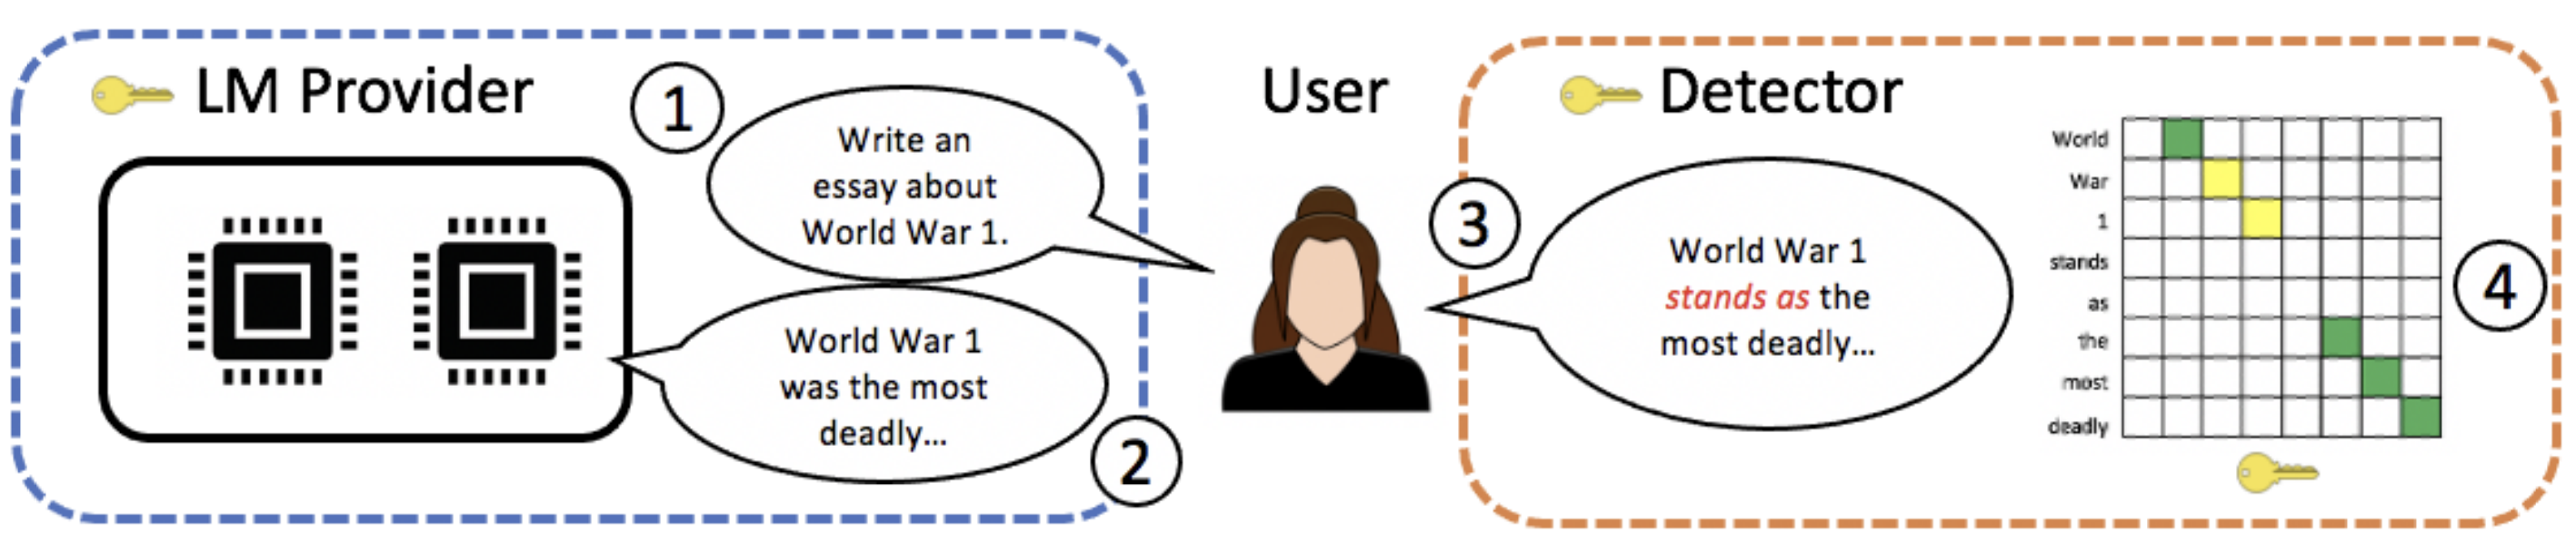
\includegraphics[width=0.8\linewidth]{./images/parties-digaram.png}
        \caption{\footnotesize Example Watermarking protocol.\cite{kuditipudi2023robustarticle}}
        \label{fig:watermarking}
    \end{figure}
    \begin{enumerate}
        \item The \textbf{User} requests a text from the \textbf{LM Provider}.
        \item The \textbf{LM Provider} generates the text and embeds a watermark using a secret key.
        \item The (malicious) \textbf{User} receives the watermarked text, edits it, and publishes it.
        \item The \textbf{Detector} receives the text and uses the secret key to check if it contains a watermark. Even if the text is edited, the watermark should still be detectable.
    \end{enumerate}
\end{frame}

\begin{frame}{Properties of an ideal Text Watermark}
    \begin{enumerate}
        \item \textbf{Distortion-free:} Preserves the model's \emph{original output distribution}. The watermark shouldn't degrade quality or bias the content.
        \item \textbf{Agnostic detection:} Can be detected \emph{without access to the original model or prompt}. There should be need to query the model or know the context.
        \item \textbf{Robust:} Should \emph{withstand perturbations} of the watermarked text such as editing, paraphrasing, cropping, or noise insertion in the text.
    \end{enumerate}
\end{frame}